\section{拟合误差与稳定性}
\label{sec:opt-fit-error}

前面每个定理给出的都是某个精确问题的精确解。实际得到的函数还受三类因素影响：读数本身有扰动，正则参数需要选择，计算只能在有限的表示中、用有限的迭代完成。这三者改变的对象不同，度量它们的范数也不同。本节固定同一个观测任务，把它们一一分开：先在固定的$\lambda$下看数据扰动怎样传到最优函数，再看$\lambda$本身怎样决定拟合程度，最后区分表示受限与计算未完成两种误差。

\subsection{固定正则参数下的数据扰动}
\label{sec:opt-fit-data-perturbation}

\paragraph{有限观测}
固定有界观测$L$、Gram矩阵$\bm G$与$\lambda>0$，比较数据$\bm y$与$\bm y+\delta\bm y$下的两个精确解。由定理~\ref{thm:opt-fit-kernel-ridge}，规范系数之差为$\delta\bm a=(\bm G+n\lambda\bm I)^{-1}\delta\bm y$，函数之差$\delta f=\sum_j\delta a_jh_j$。

\begin{theorem}[有限观测下的数据稳定性]
\label{thm:opt-fit-data-stability}
在上述设定下，
\[
  \|\delta f\|_H\le\frac{\|\delta\bm y\|_2}{2\sqrt{n\lambda}},\qquad
  \|L\,\delta f\|_2\le\|\delta\bm y\|_2 .
\]
\end{theorem}

\begin{proof}
设$\bm G=\sum_kt_k\bm u_k\bm u_k^\top$是谱分解，$t_k\ge0$，$\{\bm u_k\}$标准正交。由式~\eqref{eq:opt-fit-gram-calculus}，
\[
  \|\delta f\|_H^2=\delta\bm a^\top\bm G\,\delta\bm a=\sum_k\frac{t_k}{(t_k+n\lambda)^2}(\bm u_k^\top\delta\bm y)^2 .
\]
函数$t\mapsto t/(t+c)^2$在$t\ge0$上的最大值是$1/(4c)$，在$t=c$处取到（求导可得），取$c=n\lambda$即得第一式。读数之差$L\delta f=\bm G\delta\bm a=\sum_kt_k(t_k+n\lambda)^{-1}(\bm u_k^\top\delta\bm y)\bm u_k$，每个因子不超过$1$，得第二式。
\end{proof}

谱权重$t/(t+n\lambda)^2$解释了这个界从哪里来。很大的特征方向被数据项牢牢约束，扰动在那里被$1/t$压小；很小的特征方向被正则项压住；最危险的是$t\approx n\lambda$的中间方向，两种力量都不强。$\lambda$越小，这个最坏的放大倍数$1/(2\sqrt{n\lambda})$越大。

在例~\ref{ex:opt-fit-min-kernel}中取$\delta\bm y=(\varepsilon,0)^\top$，$n\lambda=\tfrac12$。$\delta\bm a=(\bm G+\tfrac12\bm I)^{-1}\delta\bm y=(\tfrac65,-\tfrac25)^\top\varepsilon$，$\bm G\delta\bm a=(\tfrac25,\tfrac15)^\top\varepsilon$，于是$\|\delta f\|_H^2=\delta\bm a^\top\bm G\delta\bm a=(\tfrac{12}{25}-\tfrac2{25})\varepsilon^2=0.4\varepsilon^2$，$\|\delta f\|_H\approx0.632\varepsilon$，在界$\varepsilon/\sqrt2\approx0.707\varepsilon$之内。图~\ref{fig:opt-fit-data-perturbation}在一个十二点的高斯核例子上比较两个$\lambda$：只把一个读数上移$0.4$，$\lambda=10^{-7}$时函数在扰动点两侧都出现起伏，$\|\delta f\|_H\approx16.3$；$\lambda=10^{-2}$时变化平缓而局部，$\|\delta f\|_H\approx0.33$。

\begin{figure}[!htbp]
  \centering
  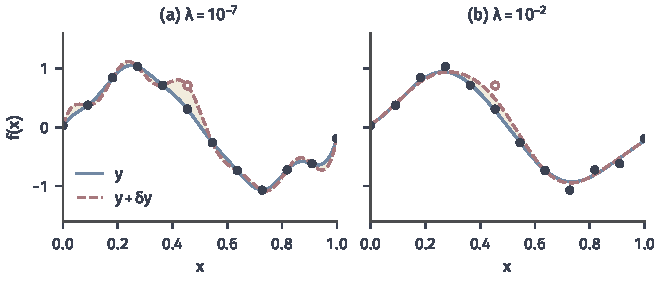
\includegraphics[width=112mm]{figures/03-optimization-evolution-and-signals/01-optimization/matplotlib/c8-data-perturbation/figure.pdf}
  \caption{固定$\lambda$下数据扰动对拟合的影响。高斯核（$\sigma=0.15$），$x_i=i/11$（$i=0,\dots,11$），教学示例读数$y_i=\sin2\pi x_i$加固定种子的$N(0,0.1^2)$噪声（黑点）；只把第六个读数上移$0.4$（空心点）。蓝线与红色虚线分别为扰动前后的核岭回归解，黄色区域为两者之差。(a)~$\lambda=10^{-7}$：$\|\delta f\|_H\approx16.3$，界$\|\delta\bm y\|_2/(2\sqrt{n\lambda})\approx183$；(b)~$\lambda=10^{-2}$：$\|\delta f\|_H\approx0.33$，界约为$0.58$。}
  \label{fig:opt-fit-data-perturbation}
\end{figure}

\paragraph{整体观测}
对第~\ref{sec:opt-fit-function-values}小节的整体观测，数据扰动$\delta y$的谱坐标$\delta c_j$经过同一个乘子：$\delta b_j=\mu_j\delta c_j/(\mu_j+\lambda)$。由此
\[
  \begin{gathered}
  \|\delta f\|_{L^2}^2=\sum_j\Bigl(\frac{\mu_j}{\mu_j+\lambda}\Bigr)^2\delta c_j^2\le\|\delta y\|_{L^2}^2,\\
  \|\delta f\|_H^2=\sum_j\frac{\mu_j}{(\mu_j+\lambda)^2}\delta c_j^2\le\frac{\|\delta y\|_{L^2}^2}{4\lambda}.
  \end{gathered}
\]
同一个扰动在两个范数下有不同的稳定常数：$L^2$中不放大，$H$中最多放大$1/(2\sqrt\lambda)$倍。原因是$H$范数给小特征值方向更重的权重$1/\mu_j$，而这些方向恰是$\lambda$小时最容易被数据带动的方向。

\paragraph{这些界比较的是什么}
两个界比较的是两个精确问题的精确解，对象、核、观测位置与$\lambda$都固定。若改变观测位置、测度或核，$\bm G$、算子乃至表示元本身都变了，需要另外控制这些对象的扰动，不能继续套用上面只针对数据的公式。求解器的舍入误差也是另一回事：它取决于线性系统$\bm G+n\lambda\bm I$的条件数，后者不超过$(t_{\max}+n\lambda)/(n\lambda)$；原问题对数据的敏感性和算法的数值稳定性应分别评价。

\subsection{正则参数与拟合程度}
\label{sec:opt-fit-lambda}

\paragraph{$\lambda\downarrow0$的极限：有限观测}
固定数据，让正则参数趋于零。在$\bm G$的特征坐标中，规范系数为$\bm a_\lambda=\sum_k(t_k+n\lambda)^{-1}(\bm u_k^\top\bm y)\bm u_k$。零特征值方向上的分量是$(n\lambda)^{-1}\bm u_k^\top\bm y$，它会发散，但由于$\ker\bm G$中的系数不改变函数，它对$f_\lambda$没有贡献。只看正特征值，令$f^\dagger=\sum_j(\bm G^\dagger\bm y)_jh_j$，
\[
  \|f_\lambda-f^\dagger\|_H^2=\sum_{t_k>0}t_k\Bigl(\frac1{t_k+n\lambda}-\frac1{t_k}\Bigr)^2(\bm u_k^\top\bm y)^2\longrightarrow0 .
\]
所以$f_\lambda\to f^\dagger$于$H$。$f^\dagger$是在所有使$\|Lf-\bm y\|_2$最小的函数中范数最小的一个：读数$\bm G\bm a$能达到的最近点是$\bm y$在$\operatorname{range}\bm G$上的投影$\bm G\bm G^\dagger\bm y$，而在读数等于它的函数中，按定理~\ref{thm:opt-fit-min-norm-interpolation}的论证，$f^\dagger$范数最小。若$\bm y\in\operatorname{range}\bm G$，$f^\dagger$就是最小范数插值，这正是图~\ref{fig:opt-fit-min-kernel}(a)中红色虚线的来历；若$\bm y\notin\operatorname{range}\bm G$，极限的残差是$\|(\bm I-\bm G\bm G^\dagger)\bm y\|_2>0$，不应称为插值。

\paragraph{$\lambda\downarrow0$的极限：整体观测}
整体观测下，$b_j^\star=\mu_jc_j/(\mu_j+\lambda)\to c_j$。在$L^2$中，$\|f_\lambda-\sum_jc_j\psi_j\|_{L^2}^2=\sum_j\bigl(\lambda c_j/(\mu_j+\lambda)\bigr)^2$，每项不超过$c_j^2$且逐项趋于零，由控制收敛（对级数），极限为零：$f_\lambda$在$L^2$中收敛到$y$在可表示方向的闭包上的投影$y-y_0$。在$H$中则不然：$\|f_\lambda\|_H^2=\sum_j\mu_jc_j^2/(\mu_j+\lambda)^2$随$\lambda\downarrow0$单调增加到$\sum_jc_j^2/\mu_j$。只有当这个和有限，即$y-y_0\in H$时，$f_\lambda$才在$H$中收敛；否则$H$范数趋于无穷。在最小值核的例子中$y=1$，$\sum_jc_j^2/\mu_j=\sum_j2=\infty$：拟合在$L^2$中趋于$1$，在$H_{\min}$中却越来越“贵”，与图~\ref{fig:opt-fit-spectral-shrinkage}(b)中越来越陡的边界层相符。这里讨论的是精确解随参数变化的极限，它和迭代算法的轨迹极限是两回事，后者在第~\ref{sec:opt-fit-implicit-bias}节讨论。

\paragraph{残差与范数的此消彼长}
固定数据，比较不同$\lambda$下的读数残差与函数范数。在$\bm G$的特征坐标中，
\[
  \bm G\bm a_\lambda-\bm y=-\sum_k\frac{n\lambda}{t_k+n\lambda}(\bm u_k^\top\bm y)\bm u_k,\qquad
  \|f_\lambda\|_H^2=\sum_k\frac{t_k}{(t_k+n\lambda)^2}(\bm u_k^\top\bm y)^2 .
\]
第一式每个系数随$\lambda$增大，第二式每项随$\lambda$减小，所以残差范数$\|Lf_\lambda-\bm y\|_2$关于$\lambda$单调不减，函数范数$\|f_\lambda\|_H$单调不增。把每个$\lambda$对应的一对数画在双对数坐标中，得到的曲线常呈“L”形，称为\term{L曲线}（L-curve）。图~\ref{fig:opt-fit-lcurve}在十五个带噪读数上画出了解族与L曲线：$\lambda=10^{-7}$时残差只有$0.07$，函数范数却达到$41$，曲线贴着每个点抖动；$\lambda=10^{-1}$时范数降到约$0.95$，残差升到$0.92$，曲线被明显压平。

\paragraph{残差匹配原则}
若事先知道读数误差的确定性上界$\|\bm e\|_2\le\delta$，一个自然的选择是不要求残差比误差更小：取$\lambda$使$\|Lf_\lambda-\bm y\|_2=\delta$。由上面的单调性和连续性，当$\|(\bm I-\bm G\bm G^\dagger)\bm y\|_2<\delta<\|\bm y\|_2$时，这样的$\lambda$存在。这一做法称为\term{残差匹配原则}（discrepancy principle）。图~\ref{fig:opt-fit-lcurve}中的教学数据是人为加噪的，误差向量已知，$\|\bm e\|_2\approx0.559$，按此原则得到$\lambda\approx2.8\times10^{-2}$（绿色），它在L曲线上位于拐角附近。实际问题中通常只有误差的估计，这时原则的结论依赖于估计是否可靠。

\begin{figure}[!htbp]
  \centering
  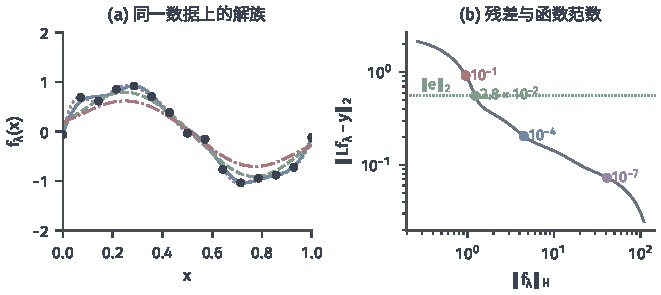
\includegraphics[width=112mm]{figures/03-optimization-evolution-and-signals/01-optimization/matplotlib/c8-lcurve/figure.pdf}
  \caption{正则参数决定拟合程度。高斯核（$\sigma=0.15$），教学示例数据为$x_i=i/14$上的$\sin2\pi x_i$加固定种子的$N(0,0.15^2)$噪声，$n=15$。(a)~$\lambda=10^{-7}$（紫色点线）、$10^{-4}$（蓝线）、$2.8\times10^{-2}$（绿色虚线）、$10^{-1}$（红色点划线）的核岭回归解。(b)~L曲线：横轴为函数范数$\|f_\lambda\|_H$，纵轴为读数残差$\|Lf_\lambda-\bm y\|_2$，均为对数刻度；圆点对应(a)中的四个$\lambda$，绿色点线为噪声范数$\|\bm e\|_2\approx0.559$，残差与之相等处即残差匹配原则选出的$\lambda$。}
  \label{fig:opt-fit-lcurve}
\end{figure}

\paragraph{这里不讨论预测保证}
无论L曲线还是残差匹配原则，都只用到训练读数和确定性的误差界。基于随机样本的交叉验证、使期望风险最小的参数以及统计一致性，需要关于数据生成机制的假设，属于统计学习理论的问题，可参考\BookChapterRef{chap:statistical-learning-framework}{卷六“机器学习理论基础”章}。不能由训练残差小推出预测误差小。

\subsection{表示误差与计算误差}
\label{sec:opt-fit-representation-computation}

\paragraph{两种差值}
固定候选空间$H$与目标$J$，记精确最优值$J^\star=\inf_HJ$。算法返回某个$\hat f$，差值$J(\hat f)-J^\star$称为优化误差，它来自算法没有解完。另一方面，若为了计算把候选限制到子空间$H_m\subseteq H$（例如$m$个特征张成的空间），即使在$H_m$中精确求解，所得最优值$J_m^\star=\inf_{H_m}J$也可能大于$J^\star$，差值$J_m^\star-J^\star\ge0$称为表示误差，它来自候选集合受限。在$H_m$中计算得到$\hat f_m$时，
\[
  J(\hat f_m)-J^\star=\underbrace{\bigl(J(\hat f_m)-J_m^\star\bigr)}_{\text{优化误差}}+\underbrace{\bigl(J_m^\star-J^\star\bigr)}_{\text{表示误差}},
\]
两项都以同一个目标值度量，所以可以相加。若关心的是函数之间的距离，就需要一个把目标值差转成距离的条件，不能把一个目标值差和一个范数距离直接相加。

\paragraph{目标值差控制函数距离}
对平方拟合目标~\eqref{eq:opt-fit-kernel-ridge}，这个条件可以精确写出。对任意$f\in H$，令$g=f-f_\lambda$，展开得
\[
  J(f_\lambda+g)=J(f_\lambda)+2\Bigl[\frac1n\langle Lf_\lambda-\bm y,Lg\rangle+\lambda\langle f_\lambda,g\rangle_H\Bigr]+\frac1n\|Lg\|_2^2+\lambda\|g\|_H^2 .
\]
方括号为零：由$L_ig=\langle g,h_i\rangle$与$f_\lambda=\sum_ja_jh_j$，它等于$\bigl\langle\sum_j[\tfrac1n(\bm G\bm a-\bm y)_j+\lambda a_j]h_j,\,g\bigr\rangle_H$，而规范系数满足$(\bm G+n\lambda\bm I)\bm a=\bm y$，括号内每个系数都是零。于是
\begin{equation}
  J(f)-J(f_\lambda)=\frac1n\|L(f-f_\lambda)\|_2^2+\lambda\|f-f_\lambda\|_H^2\ \ge\ \lambda\|f-f_\lambda\|_H^2 .
  \label{eq:opt-fit-objective-gap}
\end{equation}
任何近似解的目标值差都直接给出它到精确解的$H$距离上界，表示误差和优化误差可以先在目标值中相加，再通过这个不等式换成距离。

\paragraph{有限特征与提前停止改变不同的对象}
观测数很大时有两类常见的省算办法。一类是有限特征近似：用$m\ll n$个特征张成$H_m$，或用低秩矩阵代替$\bm G$；前者限制了候选集合，后者改变了目标本身，误差应相对于各自声明的精确问题评价。另一类是\term{提前终止}（early stopping）：在完整的$n$维系数问题上运行梯度法或CG，迭代若干轮后停下；候选集合与目标都没变，留下的是优化误差。两者都减少了计算量，但前者的误差不会随迭代增加而消失，后者的误差会；把它们都称为“近似”而不说明改变了什么，就无法判断结果相对于哪个问题可信。

\paragraph{系数误差与函数误差}
在固定的Gram矩阵下迭代求系数时，系数误差与函数误差由式~\eqref{eq:opt-fit-gram-calculus}联系：
\[
  \begin{gathered}
  \|f_{\bm a}-f_{\bm b}\|_H^2=(\bm a-\bm b)^\top\bm G(\bm a-\bm b)\le\|\bm G\|_2\,\|\bm a-\bm b\|_2^2,\\
  |L_i(f_{\bm a}-f_{\bm b})|\le\|h_i\|_H\,\|f_{\bm a}-f_{\bm b}\|_H=\sqrt{\bm G_{i,i}}\,\|f_{\bm a}-f_{\bm b}\|_H .
  \end{gathered}
\]
所以系数收敛推出函数收敛，函数收敛又推出每个读数收敛。反过来不成立：$\bm G$奇异时，系数可以沿$\ker\bm G$漂移而函数不变，例如仿射核例子中$\bm a+c(1,-2,1)^\top$对任何$c$都给出同一函数。因此停止准则应按关心的量来定：关心读数时监控$\bm G\bm a$，关心函数时监控Gram二次型，不必要求系数本身收敛。

对线性系统$(\bm G+n\lambda\bm I)\bm a=\bm y$的近似解$\bm a$，记残差$\bm s=(\bm G+n\lambda\bm I)\bm a-\bm y$。则$\bm a-\bm a_\lambda=(\bm G+n\lambda\bm I)^{-1}\bm s$，与数据扰动$\delta\bm y=\bm s$时的系数差完全相同，由定理~\ref{thm:opt-fit-data-stability}，
\[
  \|f_{\bm a}-f_\lambda\|_H\le\frac{\|\bm s\|_2}{2\sqrt{n\lambda}} .
\]
未解完的计算误差，在函数层面表现得就像一次大小为$\|\bm s\|_2$的数据扰动。在例~\ref{ex:opt-fit-min-kernel}中，若迭代停在线性残差$\bm s=(\varepsilon,0)^\top$处，上一小节的计算说明函数误差约为$0.632\varepsilon$。于是，若希望计算误差不超过数据本身的不确定性，可以要求$\|\bm s\|_2$不超过已知的读数误差量级，而不必追求机器精度。
